\documentclass[letterpaper,10pt,conference]{IEEEtran}
\usepackage{amsmath,amssymb}
\usepackage{booktabs,cite,graphicx}
\usepackage{newtxtext,newtxmath}

\newcommand{\vect}{\operatorname{vec}}
\newcommand{\unit}{\operatorname{unit}}
\newcommand{\CE}{\operatorname{CE}}

\begin{document}
\title{Preserving the Viewed Photograph in EEG-to-Image Reconstruction}
\author{\IEEEauthorblockN{Anonymous Authors}}
\maketitle

\begin{abstract}
EEG-to-image reconstruction should preserve which photograph a person viewed, even when several photographs show the same object. We train for this distinction by rendering four EEG conditions from one object concept with shared diffusion noise and enforcing bidirectional correspondence with the four source photographs. The assignment loss acts on rendered images and differentiates through the complete four-step sampler. At inference, repeat-aware EEG features provide the image condition while an EEG-predicted layout initializes sampling. On all ten THINGS-EEG2 participants with 80 repetitions, our generated images recover the exact source in 16.25\% of queries under DINOv2 scoring, compared with 7.55\% for the strongest encoder in the shared-renderer benchmark. The assignment term improves structural similarity across two repeat budgets and a concept-disjoint replication. Against four native systems, our images achieve the highest structural similarity, while identification of the depicted object remains limited.
\end{abstract}

\begin{IEEEkeywords}
Electroencephalography, visual reconstruction, conditional generation, stimulus correspondence
\end{IEEEkeywords}

\section{Introduction}

When a participant views two photographs of bicycles, their EEG responses may contain evidence of both the shared object and the differences between the photographs. An image generator can exploit the first kind of evidence and still produce nearly interchangeable outputs for the two recordings. This ambiguity matters for visual reconstruction. A plausible bicycle is an incomplete reconstruction if the response fails to distinguish the viewed photograph from another bicycle photograph.

EEG visual decoders typically learn to align a neural embedding with a pretrained visual space \cite{song2024,li2024,zheng2026}. The aligned embedding can be used for retrieval or as a diffusion condition. Retrieval from an EEG embedding and retrieval from its generated image are separate measurements. A decoder can rank the right image feature before generation, while its renderer may preserve only a subset of the features that supported the ranking. The reported utility of low-level visual features in EEG reconstruction further motivates testing structure and object identity separately \cite{yang2025}.

We supervise correspondence \emph{after rendering}. A training group contains four photographs of one object concept, together with the EEG recorded for each photograph. The generator uses the same random draws for the group. We score the correspondence of each rendered image against every source photograph and optimize the diagonal of the resulting assignment in both directions. A similarity contribution common to all pairs cancels in the assignment probabilities, which gives the loss a mechanism for targeting variation within an object concept. Repeat-aware readout and a coarse layout predicted from EEG supply the condition and initial state used by the renderer.

We evaluate the approach in two settings. A controlled comparison measures reconstructions from different encoders under a common renderer. A comparison with four native systems measures performance under a common test panel and evaluator. We isolate the assignment loss with an equal-positive-weight control, repeat the comparison on 50 disjoint concepts, and report exact-photograph retrieval and open-vocabulary object naming as separate outcomes.

\section{Related Work}

\paragraph{Visual decoding from EEG}
NICE uses contrastive alignment for EEG-based recognition \cite{song2024}. The Adaptive Thinking Mapper (ATM) maps EEG into a visual embedding and uses guided diffusion for reconstruction \cite{li2024}. Guided visual feature learning with randomized EEG trials also uses pretrained image features, with object classification as its endpoint \cite{fan2025}. Brain-HiVE learns a fused visual prior across visual representations and aligns brain activity with that prior \cite{zheng2026}. We inherit its visual target, image adapter, and projection and use comparisons among completed reconstructions to train the final image condition.

\paragraph{Diffusion-based neural reconstruction}
Psychometry aligns fMRI and images across participants and uses subject-specific memory retrieval to condition reconstruction \cite{quan2026}. CognitionCapturer combines multimodal information for decoding and image generation \cite{zhang2025}. ENIGMA employs a parameter-efficient multi-subject decoder \cite{kneeland2026}. Dual-diffusion guided EEG reconstruction studies frequency-aware encoding and reciprocal alignment between EEG and image latents \cite{yu2026}. Our supervision addresses an assignment within the same concept using the rendered RGB image and its final latent. We use a frozen SDXL-Turbo renderer \cite{sauer2024} and evaluate an EEG-derived layout as a separate input to it.

\section{Method}
\label{sec:method}

For a known participant \(s\), let \(X\) be the set of physical EEG presentations of one photograph. The model predicts a coarse latent layout \(L_s(X)\) and four image tokens \(T_s(X)\). A renderer \(G\) then produces \(\widehat I=G(L_s(X),T_s(X);\xi)\), where \(\xi\) denotes the initial and step noise. Figure~\ref{fig:method} shows which information is available during training and testing.

\begin{figure}[t]
\centering
\small
\begin{tabular}{@{}c@{}}
EEG repetitions \(X\) from participant \(s\) \\
\(\swarrow\hspace{9em}\searrow\) \\
Coarse layout \(L_s(X)\)
\qquad
Image condition \(T_s(X)\) \\
\(\searrow\hspace{9em}\swarrow\) \\
Four-step diffusion renderer \(\longrightarrow\widehat I\)
\end{tabular}
\caption{The same EEG input supplies the initial layout and image condition for one reconstruction. During training, reconstructions are assigned to source photographs within their object concept.}
\label{fig:method}
\end{figure}

\subsection{Within-concept assignment of rendered images}

Take \(K\) distinct photographs \(I_1,\ldots,I_K\) of one object concept and the EEG \(X_1,\ldots,X_K\) recorded from one participant. In the two-photo case, the total correct-pair distance \(d_{11}+d_{22}\) should be smaller than the exchanged-pair distance \(d_{12}+d_{21}\), where \(d_{ij}=1-S_{ij}\). We sample four of the ten training photographs per concept, giving each reconstruction three same-concept alternatives. Four such groups make an update of 16 complete renders. At this stage, the frozen EEG backbone reads the four-repeat average for each photograph. Training layouts are EEG predictions from ridge fits that omit the current concept fold. The layout basis is shared across the training concepts. We use identical initial and step noise across the group. For reconstructed image \(\widehat I_i\) and source \(I_j\), the similarity is
\begin{equation}
S_{ij}=0.60 S^{H/14}_{ij}+0.25 S^{B/32}_{ij}+0.15 S^{\rm layout}_{ij},
\label{eq:similarity}
\end{equation}
where the first two terms compare frozen visual features by cosine similarity and the third compares latents pooled to \(16\times16\). The visual features carry most of the weight, with a smaller contribution from direct layout similarity. We keep this scoring rule fixed in the assignment and positive-only arms. The assignment term is
\begin{equation}
\mathcal L_{\rm a}=\tfrac12\big[\CE(a S,\mathbf y)+\CE(a S^\top,\mathbf y)\big],
\quad \mathbf y=(1,\ldots,K).
\label{eq:assignment}
\end{equation}
The row term asks each reconstruction to prefer its own source. The column term asks each source to prefer its own reconstruction. The fixed logit scale \(a=15\) controls how sharply the assignment responds to score differences. For example, a 0.1 similarity gap gives a relative softmax weight of \(e^{1.5}\). We minimize
\begin{equation}
\mathcal L=\mathcal L_{\rm a}+
\tfrac12\left(1-\tfrac1K\textstyle\sum_i S_{ii}\right)
+0.05\operatorname{MSE}(T,T_{\rm init}),
\label{eq:train}
\end{equation}
where \(T_{\rm init}\) is the output of the frozen condition head at initialization. The coefficient on the positive term stays at 0.5 in the control, which isolates the effect of adding Eq.~\eqref{eq:assignment}. The quadratic penalty with weight 0.05 discourages large changes to the initial condition. We differentiate through the four denoising updates and the VAE decoder, following full-sampler optimization \cite{clark2024}, and update the EEG-dependent token residual. Before this stage, the shared EEG encoder is trained using frozen visual targets and cross-participant alignment, followed by 800 within-concept representation updates and 600 updates with matched and mismatched conditioning in the denoising objective. The final stage runs 120 updates.

\paragraph{What the assignment constrains}
Suppose a concept-specific similarity contributes an additive scalar \(b\) to every entry of \(S\). Then \(\mathcal L_{\rm a}(S+b\mathbf 1\mathbf 1^\top)=\mathcal L_{\rm a}(S)\). If the rows are identical, the column loss equals \(\log K\) and the mean row loss is at least \(\log K\) by Jensen's inequality. If every diagonal exceeds the off-diagonal entries in its row and column by \(m>0\), then \(\mathcal L_{\rm a}\leq\log(1+(K-1)e^{-am})<\log K\). The argument concerns the score matrix and gives the assignment supervision a preference for stimulus-specific variation. The positive-similarity term continues to reward similarity shared by correct pairs.

\subsection{Repeat-aware image conditioning}

Let \(x_{r,c,t}\) be the signal at repetition \(r\), channel \(c\), and sample \(t\). For a group \(B\) of four real presentations we compute the weighted waveform
\begin{equation}
\bar x_{c,t}=\frac{\sum_{r\in B}a_{r,c}x_{r,c,t}}{\sum_{r\in B}a_{r,c}},
\quad
a_{r,c}=\big[\max\big(\langle x_{r,c,t}^{2}\rangle_t,10^{-6}\big)\big]^{-1/2}.
\label{eq:repeat}
\end{equation}
The inverse RMS weights attenuate high-amplitude repeats at each channel. We use the same encoder \(E_s\) for the aggregate waveform and the individual trials. The group feature, applied to both the fused output \(f\) and hidden feature \(h\), is
\begin{equation}
\psi_B=0.72 E_s(\bar x,4)+\frac{0.28}{4}\sum_{r\in B}E_s(x_r,1).
\label{eq:fusion}
\end{equation}
Here the second argument is the effective repetition count. The aggregate waveform emphasizes responses that recur at aligned time points. Averaging features from individual trials retains a contribution from responses that may be attenuated by waveform averaging. The 0.72/0.28 mix follows the earlier repeat-readout comparison and gives the aggregate branch the larger weight. We use the same mixture for all participants and both repeat budgets. The encoder reads three fixed temporal horizons through participant-specific projections and a shared residual trunk. One group uses the four physical repeats available for each training photograph. R4 uses one group and R80 averages 20 disjoint groups.

We project the fused feature \(f\) through the frozen Brain-HiVE image adapter and projection \(A\) after training-set calibration \(C\). The calibration uses a training mean direction \(u\), scale \(r_0\), and weights \(\alpha,\beta\):
\begin{equation}
C(f)=r_0\,\unit\!\left(\alpha u+
\beta\,\unit\big[(I-uu^\top)\unit(f)\big]\right),
\end{equation}
where \(\unit\) denotes normalization with a numerical floor. The four 2,048-dimensional tokens are \(T_s=A(C(f))+R_\theta(h)\). The residual is layer-normalized, projected to width 128 with a SiLU activation, and projected back to token space. We inherit the 35\% Frobenius-norm cap from the initial condition head. It limits how much the learned residual can change the frozen adapter's output.

\subsection{EEG-predicted layout}

Let \(z_i\) be the frozen VAE representation of training photograph \(I_i\) and \(\mu\) the mean vectorized training latent. We fit a 256-dimensional basis \(U\) by emphasizing coarse spatial components while computing principal directions of \(z_i-\mu\). Predicting coefficients in this basis makes the EEG regression lower-dimensional and reserves the initial state for coarse structure. The regressions target \(U^\top(\vect(z_i)-\mu)\). For participant \(s\), \(W_{s,w}\) is a ridge fit from standardized EEG features in temporal window \(w\) to these coefficients. The five windows in stored samples are \(12{:}62\), \(10{:}75\), \(15{:}90\), \(10{:}125\), and \(0{:}250\). With standardized window feature \(b_{s,w}(X)\), the layout is
\begin{equation}
\vect(L_s(X))=\mu+\gamma_s U\frac{1}{5}\sum_{w=1}^5 W_{s,w}^{\top}b_{s,w}(X).
\label{eq:layout}
\end{equation}
The layout uses the weighted waveform in Eq.~\eqref{eq:repeat}, averaged over groups when applicable. We choose \(\gamma_s\) from training-concept calibration predictions. It scales their pooled low-frequency RMS to 80\% of the corresponding source-latent RMS, attenuating the regressed layout before sampling. The final regression weights are fitted on the full registered training split.

We initialize the sampler at \(L_s+\sigma_0\epsilon_0\). After the first Euler ancestral update produces \(z_1^{\rm gen}\), the next state is
\begin{equation}
z_1=0.25z_1^{\rm gen}+0.75(L_s+\sigma_1\epsilon_0).
\end{equation}
A development comparison on four participants informed the anchoring schedule. Reducing the anchor from a full first-step reset with a second-step blend to the 0.75 first-step blend raised ten-photo matching from 18.45\% to 19.95\% for the preceding decoder. The revised schedule simultaneously halves the two late correction gains. The comparison supports the schedule as a whole. The second update proceeds directly. After the third and fourth updates we add \(g_t P_8(L_s+\sigma_t\epsilon_0-z_t^{\rm gen})\), with \(g_t=0.11,0.02\). Here \(P_8\) averages \(8\times8\) latent neighborhoods and bilinearly restores the sampling resolution. All four updates receive the same tokens and an empty text prompt. The final latent decodes to one \(512\times512\) RGB image.

\begin{table*}[t]
\centering
\caption{Common-renderer reconstruction on the official THINGS-EEG2 panel. Each row summarizes 2,000 generated images. Naming and exact-photograph rank-one accuracy are percentages. Bold indicates the best point estimate within each repeat budget.}
\label{tab:common}
\small
\setlength{\tabcolsep}{2.8pt}
\begin{tabular}{llrrrrrrrrrrrr}
\toprule
 & & \multicolumn{2}{c}{Name$\uparrow$} & \multicolumn{2}{c}{Photo$\uparrow$} & & & & & & & & \\
\cmidrule(lr){3-4}\cmidrule(lr){5-6}
Repeats & EEG decoder & CLIP & SigLIP~2 & CLIP & DINOv2 & PixCorr$\uparrow$ & SSIM$\uparrow$ & Alex(2)$\uparrow$ & Alex(5)$\uparrow$ & Incep.$\uparrow$ & CLIP-2$\uparrow$ & EffNet$\downarrow$ & SwAV$\downarrow$ \\
\midrule
4 & Brain-HiVE & 0.35 & 0.500 & 3.05 & 4.45 & .1647 & .3719 & .7518 & .7684 & .6105 & .6495 & .9459 & .6356 \\
4 & ATM & 0.40 & 0.363 & 3.20 & 3.85 & .1608 & .3592 & .7397 & .7564 & .6009 & .6336 & .9515 & .6438 \\
4 & NICE & 0.45 & 0.363 & 3.10 & 3.20 & .1580 & .3613 & .7220 & .7459 & .5985 & .6274 & .9537 & .6439 \\
4 & EEGNet & 0.20 & 0.450 & 2.90 & 3.90 & .1580 & .3529 & .7250 & .7486 & .5910 & .6311 & .9532 & .6443 \\
4 & Ridge & 0.30 & 0.150 & 1.25 & 1.55 & .1719 & .3998 & .6644 & .6676 & .5524 & .5722 & .9494 & .6186 \\
4 & Ours & \textbf{1.00} & \textbf{0.925} & \textbf{6.40} & \textbf{8.20} & \textbf{.1883} & \textbf{.4182} & \textbf{.7911} & \textbf{.8201} & \textbf{.6715} & \textbf{.7073} & \textbf{.9089} & \textbf{.5830} \\
\midrule
80 & Brain-HiVE & 0.95 & 1.325 & 6.45 & 7.55 & .1862 & .3617 & .8009 & .8441 & .6719 & .7284 & .9176 & .5952 \\
80 & ATM & 0.50 & 0.562 & 4.85 & 5.55 & .1761 & .3520 & .7812 & .8233 & .6418 & .6916 & .9331 & .6147 \\
80 & NICE & 0.80 & 0.462 & 4.25 & 5.20 & .1671 & .3488 & .7686 & .8165 & .6420 & .6843 & .9352 & .6108 \\
80 & EEGNet & 0.40 & 0.462 & 3.90 & 3.95 & .1745 & .3549 & .7575 & .7996 & .6140 & .6709 & .9435 & .6152 \\
80 & Ridge & 0.35 & 0.350 & 1.30 & 1.85 & .1817 & .3968 & .6616 & .6717 & .5623 & .5771 & .9482 & .6146 \\
80 & Ours & \textbf{2.40} & \textbf{2.075} & \textbf{11.45} & \textbf{16.25} & \textbf{.2384} & \textbf{.4267} & \textbf{.8769} & \textbf{.9158} & \textbf{.7782} & \textbf{.7990} & \textbf{.8540} & \textbf{.5272} \\
\bottomrule
\end{tabular}
\end{table*}

\begin{table*}[t]
\centering
\caption{Native-system R80 reconstructions, re-scored on the same 2,000 participant-stimulus queries per row. Naming and exact-photograph rank-one accuracy are percentages. Superscripts indicate author-provided outputs (A) or our reproduction (R). Bold indicates the best point estimate.}
\label{tab:native}
\small
\setlength{\tabcolsep}{3.2pt}
\begin{tabular}{lrrrrrrrrrrrr}
\toprule
 & \multicolumn{2}{c}{Name$\uparrow$} & \multicolumn{2}{c}{Photo$\uparrow$} & & & & & & & & \\
\cmidrule(lr){2-3}\cmidrule(lr){4-5}
System & CLIP & SigLIP~2 & CLIP & DINOv2 & PixCorr$\uparrow$ & SSIM$\uparrow$ & Alex(2)$\uparrow$ & Alex(5)$\uparrow$ & Incep.$\uparrow$ & CLIP-2$\uparrow$ & EffNet$\downarrow$ & SwAV$\downarrow$ \\
\midrule
ATM$^{\rm A}$ & 1.050 & 1.375 & 7.20 & 9.20 & .1314 & .3142 & .7613 & .8353 & .6922 & .7399 & .9026 & .5906 \\
CognitionCapturer$^{\rm A}$ & .550 & .713 & 5.15 & 7.05 & .1509 & .3565 & .7546 & .8127 & .6699 & .7159 & .9096 & .5887 \\
Brain-HiVE$^{\rm R}$ & 2.025 & \textbf{2.275} & 12.05 & 13.45 & .1951 & .3288 & .8330 & .8948 & .7476 & .7998 & .8783 & .5654 \\
ENIGMA$^{\rm R}$ & 1.913 & 1.975 & \textbf{13.15} & \textbf{16.20} & .1818 & .3319 & .8473 & .9069 & .7716 & \textbf{.8256} & .8675 & .5430 \\
Ours & \textbf{2.550} & 2.075 & 11.40 & 16.15 & \textbf{.2384} & \textbf{.4267} & \textbf{.8769} & \textbf{.9158} & \textbf{.7786} & .7992 & \textbf{.8540} & \textbf{.5272} \\
\bottomrule
\end{tabular}
\end{table*}

\section{Experiments}
\label{sec:results}

\subsection{Protocol}

\paragraph{Data and inputs}
THINGS-EEG2 contains 10 participants with responses to natural photographs \cite{gifford2022}. The registered training split has 1,323 concepts and 13,230 distinct photographs. The official test comprises all 200 disjoint object concepts, one photograph per concept and 2,000 queries across participants. At test time we specify the current participant and supply 17 posterior EEG channels sampled at 250~Hz. R4 uses the first four physical repeats and R80 uses all 80 physical repeats. We also evaluate 50 training-disjoint concepts with ten photographs each, totaling 5,000 R4 queries. Photograph and category information enter scoring after rendering. All of our comparisons use one output per query.

\paragraph{Evaluation}
We follow the standard pixel and feature reconstruction measures used by ATM \cite{li2024}. PixCorr is the pixel correlation with the source and SSIM compares local image structure \cite{wang2004}. AlexNet layers 2 and 5, Inception, and CLIP use two-way comparisons between the source and distractors. EfficientNet and SwAV are feature correlation distances. In exact-photograph retrieval, the evaluator ranks the 200 source photographs by similarity to the \emph{generated image}. Open-vocabulary naming ranks 1,854 THINGS concept entries from the generated image using frozen CLIP \cite{radford2021} or SigLIP~2 \cite{tschannen2025}. Tied names share credit. DINOv2 \cite{oquab2024} provides an independent exact-photograph ranker. We compute paired 95\% intervals using 10,000 resamples over participants and stimuli.

\paragraph{Comparisons}
The common-renderer experiment adapts Brain-HiVE's BrainMLP, ATM, NICE, an EEGNet-style encoder \cite{lawhern2018}, and linear ridge to the same registered training split, image targets, visual adapter, latent-layout checkpoint, empty prompt, seeds, and four-step sampler. The four learned baseline encoders make 25 passes over training photographs through a rotating participant schedule. Ridge uses a closed-form fit. Our method uses its staged training procedure. In native-system comparison we score ATM and CognitionCapturer author outputs, plus participant-specific reproductions of Brain-HiVE and ENIGMA, on the same full official R80 panel. Native model training and sampling settings follow their respective pipelines. These two comparisons address the controlled encoder setting and the available end-to-end systems.

\begin{figure*}[t]
\centering
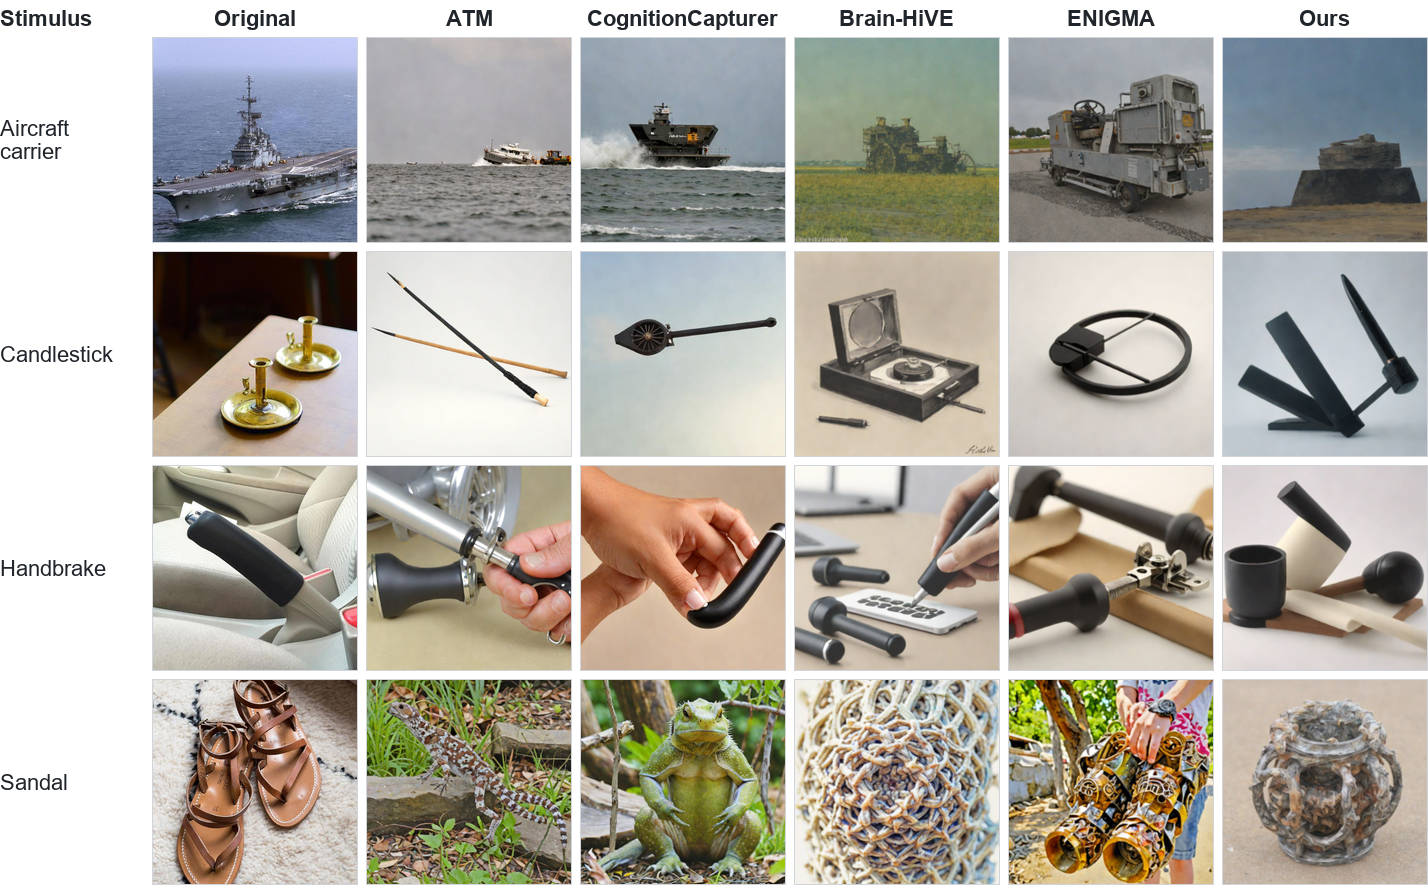
\includegraphics[width=.97\textwidth]{fixed-panel.png}
\caption{Four fixed official R80 stimuli for participant 01. Each row shows the original photograph and registered single outputs from the five systems. The panel includes correspondence and recognition failures. Images are resized for display.}
\label{fig:images}
\end{figure*}

\subsection{Reconstruction results}

\paragraph{Common renderer}
Table~\ref{tab:common} reports twelve measures. With four repeats, CLIP recovers the exact photograph for 128 of our 2,000 queries, compared with 64 for ATM. The paired gain is 3.20 percentage points (95\% interval [1.20, 5.35]). At 80 repeats, CLIP retrieves 229 originals for our method and 129 for Brain-HiVE, a gain of 5.00 points [1.50, 8.50]. On the same renders, DINOv2 recovers 8.20\% and 16.25\% of the originals under R4 and R80. The corresponding gains over Brain-HiVE are 3.75 points [1.05, 6.70] and 8.70 points [5.25, 12.30]. With R80, SigLIP~2 gives 2.075\% naming credit to our images and 1.325\% to Brain-HiVE's images. The paired difference is 0.75 points [$-0.625$, 2.25], with low absolute naming for both decoders.

\paragraph{Native systems}
Table~\ref{tab:native} retains the published or reproduced sampling pipeline for each system. Our model obtains 0.4267 SSIM, compared with 0.3288 for Brain-HiVE, a paired improvement of 0.0979 [0.0891, 0.1071]. ENIGMA leads in CLIP photograph retrieval and CLIP two-way identification. The paired differences against Brain-HiVE and ENIGMA for naming and both photograph rankers include zero. CLIP and SigLIP~2 name 85.125\% and 88.625\% of the true test photographs, respectively. Those reference scores and the low naming rates of reconstructions show the gap between photographic structure and recognizable object identity. Figure~\ref{fig:images} illustrates this gap on fixed stimuli. The handbrake reconstruction retains a dark diagonal over a bright region, while the sandal reconstruction shows a different object.

\subsection{Does assignment contribute beyond positive matching?}

We remove Eq.~\eqref{eq:assignment} while retaining the weight of the diagonal term, its initialization, and the training and rendering budgets. Table~\ref{tab:ablation} reports paired SSIM differences for three full panels. The gains hold for both repeat budgets and the 50-concept replication. On official R80, dual naming credit changes by \(+0.70\) points [\(-0.10\), \(1.60\)] and DINOv2 exact-photograph retrieval changes by \(-1.95\) points [\(-4.75\), \(0.80\)]. These intervals delimit what the assignment ablation establishes.

We also evaluated two training variants with 2,000 generated development images per arm. Averaging the layout across the training quartet lowered SSIM by 0.00489 [$-0.00656$, $-0.00329$]. Subtracting scores from images rendered with the same layout and a fixed visual condition changed SSIM by $+0.00055$ [$-0.00051$, 0.00170] and naming by $-0.40$ points [$-1.90$, 0.70]. We retain per-photograph layouts and the original assignment scores.

\begin{table}[t]
\centering
\caption{SSIM gain from adding assignment at a fixed positive-loss weight. Intervals are paired by subject and stimulus.}
\label{tab:ablation}
\small
\begin{tabular}{@{}lrc@{}}
\toprule
Test panel & \(N\) & Gain [95\% interval] \\
\midrule
Official R4 & 2,000 & \(+.0132~[+.0111,+.0153]\) \\
Disjoint 50 concepts, R4 & 5,000 & \(+.0125~[+.0108,+.0142]\) \\
Official R80 & 2,000 & \(+.0122~[+.0101,+.0144]\) \\
\bottomrule
\end{tabular}
\end{table}

\paragraph{EEG input controls}
Replacing the layout with a noise-only start in a matched R4 replay reduces SSIM from 0.4182 to 0.4010. Keeping the layout and replacing repeat-aware token estimation with arithmetic waveform averaging lowers CLIP photograph retrieval from 6.30\% to 5.20\%. Cycling EEG across stimuli within each participant reduces photograph retrieval to 0.20\%. These experiments test the sensitivity to recorded EEG and distinguish the role of the layout in structure from that of the image condition. The replay evaluates the component controls within one set of generated images.

\section{Discussion and Conclusion}

Optimizing same-concept assignment on the rendered outputs increases structural similarity in the official and disjoint panels. Exact-photograph retrieval improves under the controlled renderer, and the native-system results quantify the trade-off between reconstruction structure and object recognition. Recognition remains an open problem. A correct source photograph may rank first based on layout or texture even when the generated image depicts a different object. In our R80 native-system evaluation, 18 of the 228 correct CLIP photograph matches are also named correctly by both evaluators.

The participant-specific fit assumes training data for every test participant. This study measures stimulus fidelity using image-based metrics. Human recognition remains unmeasured. The public official test set was used for earlier comparisons and diagnostics. The 50-concept replication tests transfer of the locked assignment comparison within the same dataset. Additional independent recordings would be needed to evaluate generalization beyond that scope.

\section*{Acknowledgment}
OpenAI Codex assisted in drafting the manuscript text and the method diagram from the authors' implementation and experiment records. All reported scores are from the recorded evaluations.

\bibliographystyle{IEEEtran}
\bibliography{references}
\end{document}
